\section{Introduction}
\label{sec:intrp}

In the early 1980's, the British Broadcasting Corporation (BBC)
introduced a whole generation of educators and students in the United Kingdon (UK) 
to computing through the {\em BBC Computer Literacy Project}, which featured the BBC Micro, 
a 6502-based personal computer designed and produced by Acorn Computers Ltd. (referred
to at times as the ``British Apple'').  The project was very sucessful:
more than 80\% of UK classrooms had a BBC Micro and many of today's 
computing professionals from the UK first encountered computing through
the BBC Micro.

Fast forward to the 21st century: the BBC sought to again inspire a new
generation get creative with coding, programming and digital technology
through its 2015 {\em Make It Digital} initiative, as well as to support the UK's mandate to 
teach computer science concepts at all grade levels.~\cite{PeytonJones2013ICFP}

As part of this effort, the BBC introduced the micro:bit (see 
Figure~\ref{fig:microbit}),
a small programmable and embeddable computer designed, 
developed and deployed by the BBC and partners (including ARM, Microsoft
and Lancaster University) to approximately 800,000 UK middle school students
in 2015-2016. Harkening back to its work with the BBC Micro,
the BBC described the micro:bit as its ``most ambitious education initiative in 30 years, 
with an ambition to inspire digital creativity and 
develop a new generation of tech pioneers.''~\cite{BBCwebsite}

From a local educational experiment in the UK, the micro:bit has become
wildly successful globally because of a unique combination of hardware and
software, embracing a constructionist~\cite{Papert} approach to computing education.
Driving the worldwide expansion is
the Micro:bit Educational Foundation (\url{www.microbit.org}),
a non-profit organization
established in September 2016, with the support of its founding partners~\footnote{ARM,
Amazon, BBC, British Council, IET, Lancaster University, Microsoft,
Nominet, and Samsung.}. 
The Foundation's Mission Statement is to: 
\begin{itemize}
\item  enable and inspire all children to participate in the digital world, 
with particular focus on girls and those from disadvantaged groups.
\item make micro:bit the easiest and most effective learning tool for digital skills and creativity.
\item work in collaboration with educators to create and curate exceptional 
curriculum materials, training programmes and resources.
\item build and support communities of educators and partners 
to remove the barriers to learning digital skills
\end{itemize}

In this paper, we describe the key decisions and lessons from
delivering the BBC micro:bit in the UK and then expanding to reach 
more educators and students around the world.
We draw from two full years of 
full deployment of the micro:bit in the UK, as well as deployments
in Europe, the Americas, and Asia.  There are approximately
two million micro:bits now in the market and many hardware,
content, and education partners participating. 

%Purpose
%- what is the micro:bit?
% http://www.bbc.co.uk/programmes/articles/4hVG2Br1W1LKCmw8nSm9WnQ/the-bbc-micro-bit


% reference the competition and show what's different (hardware)
% https://barrettsprojects.wordpress.com/2012/09/15/tap-and-double-tap/ 

\begin{figure} 
  \begin{tabular}{cc}
    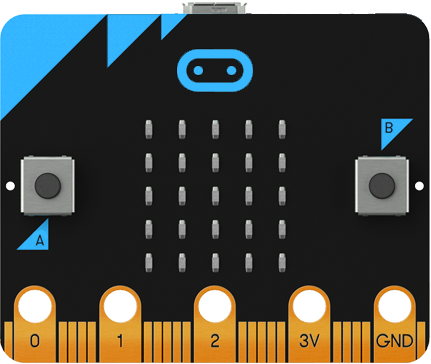
\includegraphics[width=1.5in]{images/microbit-front.png} &
    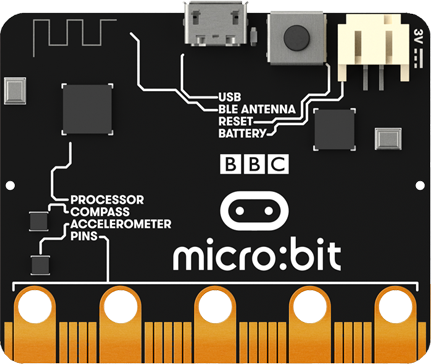
\includegraphics[width=1.5in]{images/microbit-back.png} \\
    (a) & (b) 
  \end{tabular}
  \caption{\label{fig:microbit}The micro:bit: (a) front, with two buttons, 
    5x5 LED display, and edge connector (bottom); (b) back, with processor, accelerometer, compass, Bluetooth, USB and battery ports.}
  \end{figure}
  
  \begin{figure*}[t] 
    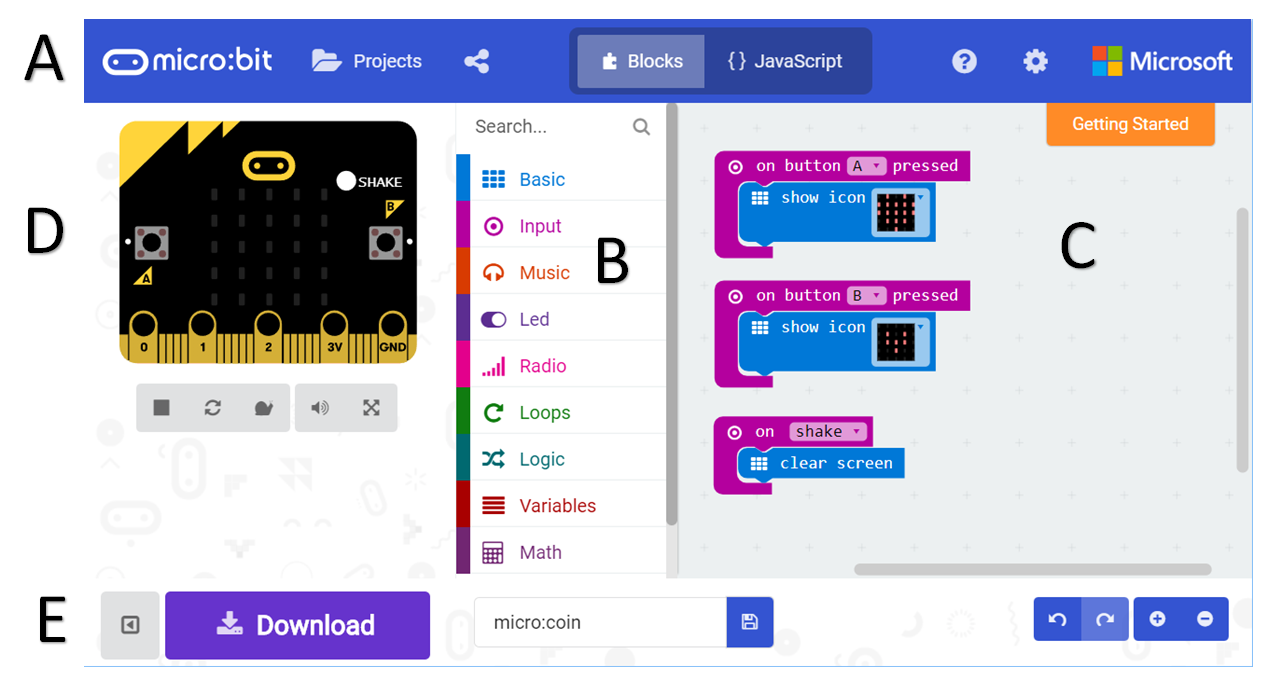
\includegraphics[width=6in]{images/webApp.png}
    \caption{\label{fig:snapshot}MakeCode web app for the micro:bit (\url{http://makecode.microbit.org}).}
  \end{figure*}

\subsection{Hardware}

Figure~\ref{fig:microbit} shows (a) the front and (b) the back of the
micro:bit, which measures 4cm x 5cm. Like the Arduino Uno~\cite{Arduino}, 
the micro:bit is a single-board microcontroller 
that can be programmed via a host computer (usually a laptop or desktop)
and then embedded in projects where it runs on battery power.
In contrast to the Uno, which has no built-in sensors, the micro:bit 
board hosts a variety of sensors (temperature, accelerometer, magnetometer, 
light level), 
a 5x5 LED matrix, two user-defined buttons, as well as Bluetooth
Low Energy (BLE) communications.\footnote{The micro:bit has a whopping
16kB of RAM and 256kB of Flash memory, compared to the Uno's 2kB of 
RAM and 32kB of Flash}.

The design of the micro:bit hardware was driven by the
first two objectives of the BBC micro:bit project:
(B1) to provide a simple creative experience for physical computing, wearable and Internet of Things (IoT) projects;
(B2) to supply a device that can continue to provide learning opportunities as the user's expertise grows.

On the hardware side, the micro:bit's built-in sensors, buttons and LED display 
allow many projects to be completed with no additional hardware or wiring. 
The holes on micro:bit's edge
connector allows additional external sensors and actuators to be connected via crocodile clips.
The micro:bit's BLE capabilities introduces networking to the
picture, and enables streaming of data and command/control operations among the micro:bit, 
smartphones, laptops, as well as other micro:bits.
As with Arduino, an ecosytem of micro:bit shields
(hardware peripherals) that accommodate the micro:bit's edge
connector expands its capabilities greatly (\url{http://microbit.org/resellers/}).

\subsection{Software}

The design of the micro:bit coding tools also was oriented towards a 
simple starting experience with room for progression. In particular, the coding 
objectives of the project were: (B3)
to give students an exciting, engaging introduction to coding;
(B4) to stimulate curiosity about how computing technologies can be utilized 
  to solve problems that students identify. 

Based on in-school trials with a micro:bit prototype, the BBC focused on delivering a web app 
based on the popular Blockly framework~\cite{Blocky2015} to permit students to
create scripts via drag-and-drop operations in a web browser, and see
the execution of their scripts via a simulator.
Text-based coding via scripting languages also 
was identified as an important feature. As the micro:bit would be incorporated 
into standalone projects, it also was essential for the user's program to be 
compiled and installed in non-volatile storage on the micro:bit where it 
could be run via battery power.

%final design put the entire toolchain in web app, without need to invoke C/C++ compiler to
%compile the user's program; ARM DAPlink solution makes micro:bit appear as USB pen drive
%on all operating systems; MicroPython provided second programming solution with entire toolchain
%on the micro:bit!!]

% less techy here

The solution delivered by the BBC's partners evolved from the initial
design to include support for Blockly, JavaScript and Python, all 
via web apps. 
Figure~\ref{fig:snapshot} shows a screen snapshot of the MakeCode web app
for the micro:bit, 
which supports programming via both Blocky and JavaScript.
The web app has five main sections: (A) menu bar with access to projects
and examples, and switching between Blockly and JavaScript editors; (B)
Blockly toolbox of micro:bit API categories; (C) Blockly programming
canvas with a simple reactive program; (D) micro:bit simulator for execution
of the user's program in browser; (E) download button, which invokes the in-browser
compiler/linker to produce a binary executable. 

% The event-based program shown in section (C) displays a large heart when the
% A button is pressed, displays a small heart when button B is pressed,
% and clears the display when the user shakes the micro:bit (shake
% detection is implemented using the accelerometer; in the simulator, the
% shake event is fired using a virtual button). In addition to event-based
% APIs, direct access to the micro:bit's sensors via polling is possible.

The Python solution for the micro:bit is based on MicroPython (\url{http://micropython.org})
an implementation of Python 3.0 for microcontrollers. It includes 
a full Python compiler and runtime that runs on the micro:bit and
supports a read-eval-print loop (REPL) to execute commands sent via 
a terminal, as well as to import and run scripts from the Python web app for 
the micro:bit (\url{http://python.microbit.org}).

% \begin{itemize}
% \item 
% \item an efficient C++ runtime for the micro:bit created by Lancaster
% University;
% \item a web app 
% with Blockly and JavaScript editors, micro:bit simulator, 
% and a compiler to machine code (linked against a pre-compiled 
% C++ runtime image, so no C++ compiler is needed for user code);
% \item a Python compiler and read-eval-print loop (REPL) that resides
% {\em on the micro:bit} (via \url{https://micropython.org/}), 
% supported by a simple web app (\url{http://python.microbit.org}) and 
% an installable application (\url{https://codewith.mu/});
% \item ARM's DAPlink firmware makes the micro:bit appear as USB pen drive 
% on most operating systems, enabling a simple file copy operation to 
% install a user's program on the micro:bit (no device drivers needed).
% \end{itemize}
% MakeCode, MicroPython, and the C++ runtime are all open source.\footnote{
% At \url{https://github.com/microsoft/pxt},
% \url{https://github.com/micropython/micropython},
% and \url{https://github.com/lancaster-university/microbit-dal}, 
% respectively.}


% \subsection{Content and training}

% The BBC micro:bit project also called for partners to develop content
% and to ``train the trainers'' (educators) around the micro:bit computing
% system.  This built on efforts by the non-profit Computing At Schools
% (\url{www.cas.org}) organization to train UK educators to teach computer
% science. 

%- A lot of lessons learned from delivering end-to-end experience in UK and other countries
%   - hardware (unique design, as already mentioned)
%   - firmware:  high-level C/C++ runtime and ARM's DAPlink
%   - web-based IDE: no C/C++ compiler needed to compile user code
%   - content
%   - training
% In country partnerships

% main points
% - mass participation
% - country readiness (or perhaps willingness)

\subsection{Overview}

Section~\ref{sec:physical} reviews physical computing, which anchors 
and defines the micro:bit experience. Section~\ref{sec:projects}
presents a broad set of micro:bit-based projects, ranging
from wearable games to environment science, that demonstrate
the micro:bit's capabilities.  Section~\ref{sec:country}
describes the rollout of the micro:bit in the UK and other countries
in Europe, the Americas and Asia. Section~\ref{sec:conclude}
concludes with final thoughts about what has made the micro:bit
successful to date and what comes next. 


% compared to Arduino
% https://twitter.com/adamwwolf/status/1019070808038072320

% success of micro:bit due to 
% - Low-cost, simplicity
% - Partnerships (hardware, software, content, training)
% - Open Source of software (CODAL, MakeCode, ...)
% - Hardware Reference design

% - why is it interesting?
%   - edge/physical/IoT computing
%   - build off of Scratch/Blockly, but untethered (via in-browser compiler)
%   - transition to JavaScript and Python

% - BBC rollout in UK
% - Global reach
%    - BBC rollout mirrored in other countries
%    - Communities
%      - Sri Lanka user group: http://microbitslug.org/
%      - UK libraries (loan program)
%    - third party editors









